\documentclass[11pt,addpoints]{exam}

\usepackage{amsmath}
\usepackage{amssymb}

\usepackage{graphicx}
\usepackage[usenames,dvipsnames]{color}

\usepackage[utf8]{inputenc}
\usepackage[T1]{fontenc}
\usepackage{lmodern} % load a font with all the characters


% Bold the 'Figure #' in the caption and separate it with a period
% Captions will be left justified
\usepackage[labelfont=bf,labelsep=period,justification=raggedright]{caption}
%\usepackage{here}

\title{Examen Cours ES2: Introduction à la bioinformatique et la génomique}
\author{Chloé-Agathe Azencott, Thomas Walter}
\begin{document}
\maketitle 

\begin{questions}

\section{Questions sur le cours}

\question[2] Notions en Biologie. 
\begin{parts}
\part Citer trois fonctions de protéines. 
\part Expliquer pourquoi un codon est constitué de trois nucléotides. 
\part Expliquer le principe de l'ARN interférence.
\part Classer les mutations selon leur effet. 
\end{parts}

\question[1] La microscopie.
\begin{parts}
\part Qu'est-ce qu'on entend par la résolution d'un microscope~? 
\part Décrire deux façons d'augmenter la résolution d'un microscope. 
\end{parts}

\question[3] Vous êtes consulté comme expert d'analyse d'images par
des biologistes qui veulent analyser une série d'expériences. Ils
utilisent un marqueur qui est informatif pour la compaction de la
chromatine, et ils cherchent à trouver des molécules spécifiques pour
rompre cette organisation. Dans les figure \ref{fig:tsa}.a et
\ref{fig:tsa}.b, nous pouvons observer des images représentatives pour
des cellules normales (sans traitement) et dans les figures
\ref{fig:tsa}.c et \ref{fig:tsa}.d nous pouvons observer l'effet d'une
molécule. Nous ajoutons que la taille et l'intensité moyenne des
cellules n'ont pas de raison d'être différentes entre les deux
conditions. 

Proposer un descripteur spécifique qui nous permettrait de quantifier
cet effet et expliquer votre choix. 

\begin{figure}[!ht]
\centering
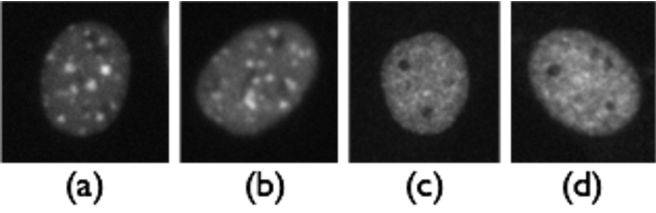
\includegraphics[scale=0.8]{TSA_phenotype.pdf}
\caption{Phenotypic readout on heterochromatin formation: (a)-(b)
  Negative Control, (c)-(d) Signal as observed 
  by an active drug.}
\label{fig:tsa}
\end{figure}

\question[4] Les descripteurs Haralick.
Les descripteurs de Haralick sont définis à partir de la matrice de
co-occurence normalisée $P_{\Delta_x}$. Nous rappelons que chaque élément
$P_{\Delta_x}(i,j)$ de cette matrice est la probabilité jointe
d'observer les valeurs de gris $i$ et $j$ pour des paires de pixels
$(x,x+\Delta_x)$ et $(x,x-\Delta_x)$, avec $Delta_x \in
\mathbb{Z}^2$. Plus formellement :  
\begin{eqnarray*}
C_{\Delta_x}(i,j) &=& |\{(x,y) \,\,| \,\, y=x \pm \Delta_x, \,\, f(x)=i,
\,\, f(y)=j \}| \\
P_{\Delta_x}(i,j) &=& \frac{C_{\Delta_x}(i,j)}{\sum_i\sum_j C_{\Delta_x}(i,j)}
\end{eqnarray*} 


Le descripteur de ``contraste'' est défini de manière suivante: 
\begin{equation}\label{equ:haralick_contrast}
\vartheta_{\Delta_x} = \sum_i\sum_j(i-j)^2P_{\Delta_x}(i,j)
\end{equation}

\begin{parts}
\part Expliquer ce que le descripteur $\vartheta_{\Delta_x}$ mesure. 
\part Ordonner les images dans la figure \ref{fig:haralick} pour (i)
$\Delta_x=(1,0)$ et (ii) la matrice moyennée pour $\Delta_x\in
\{(1,0), (0,1)\}$ (c'est-à-dire en direction horizontale et
verticale).  

Par exemple, si le descripteur était ``le nombre de pixels noirs'', on
obtiendrait la solution 1. a - 2. (b,c,d,f) - 3. e. 
\end{parts}

\begin{figure}[!ht]
\centering
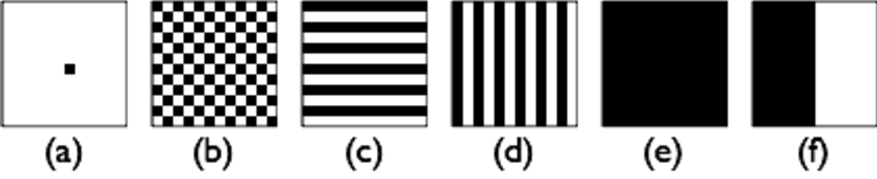
\includegraphics[scale=0.8]{Haralick_question.pdf}
\caption{Images à ordonner selon le descripteur
  \ref{equ:haralick_contrast} }. 
\label{fig:haralick}
\end{figure}


\question[4] Les chaines de Markov cachées. 
Beaucoup d'algorithmes autour des chaines de Markov cachées sont basés
sur le calcul récursif de certaines probabilités, dont : 
\begin{equation}\label{equ:alpha}
\alpha_t(i) = P(O_1\ldots O_t, q_t=S_i) 
\end{equation}
Ici, $O_t$ est l'observation au temps $t$, $q_t$ est l'état caché au
temps $t$ avec $q_t \in \{S_i\}_{i=1 \ldots N}$ (voire aussi figure
\ref{fig:hmm}).

\begin{parts}
\part Montrer que $\alpha_1(i)=\pi_i b_i(O_t)$. 
\part Montrer que $\alpha_{t+1}(j) = \left[
  \sum_{i=1}^{N}\alpha_t(i)a_{ij} \right]b_j(O_{t+1})$. 
\part Montrer que $P(O_1, \ldots O_{T}) = \sum_{i=1}^N\alpha_T(i)$. 

(Notation: $\pi_i = P(q_1=S_i)$ est la probabilité initiale pour état $S_i$,
$a_{ij} = P(q_{t+1}=S_j | q_t=S_i) $ la probabilité de transition,
$b_i(O_t) = P(O_t | q_t=S_i)$ la probabilité d'émission et $T$ la
longueur de la séquence.) 
\end{parts}

\begin{figure}[!ht]
\centering
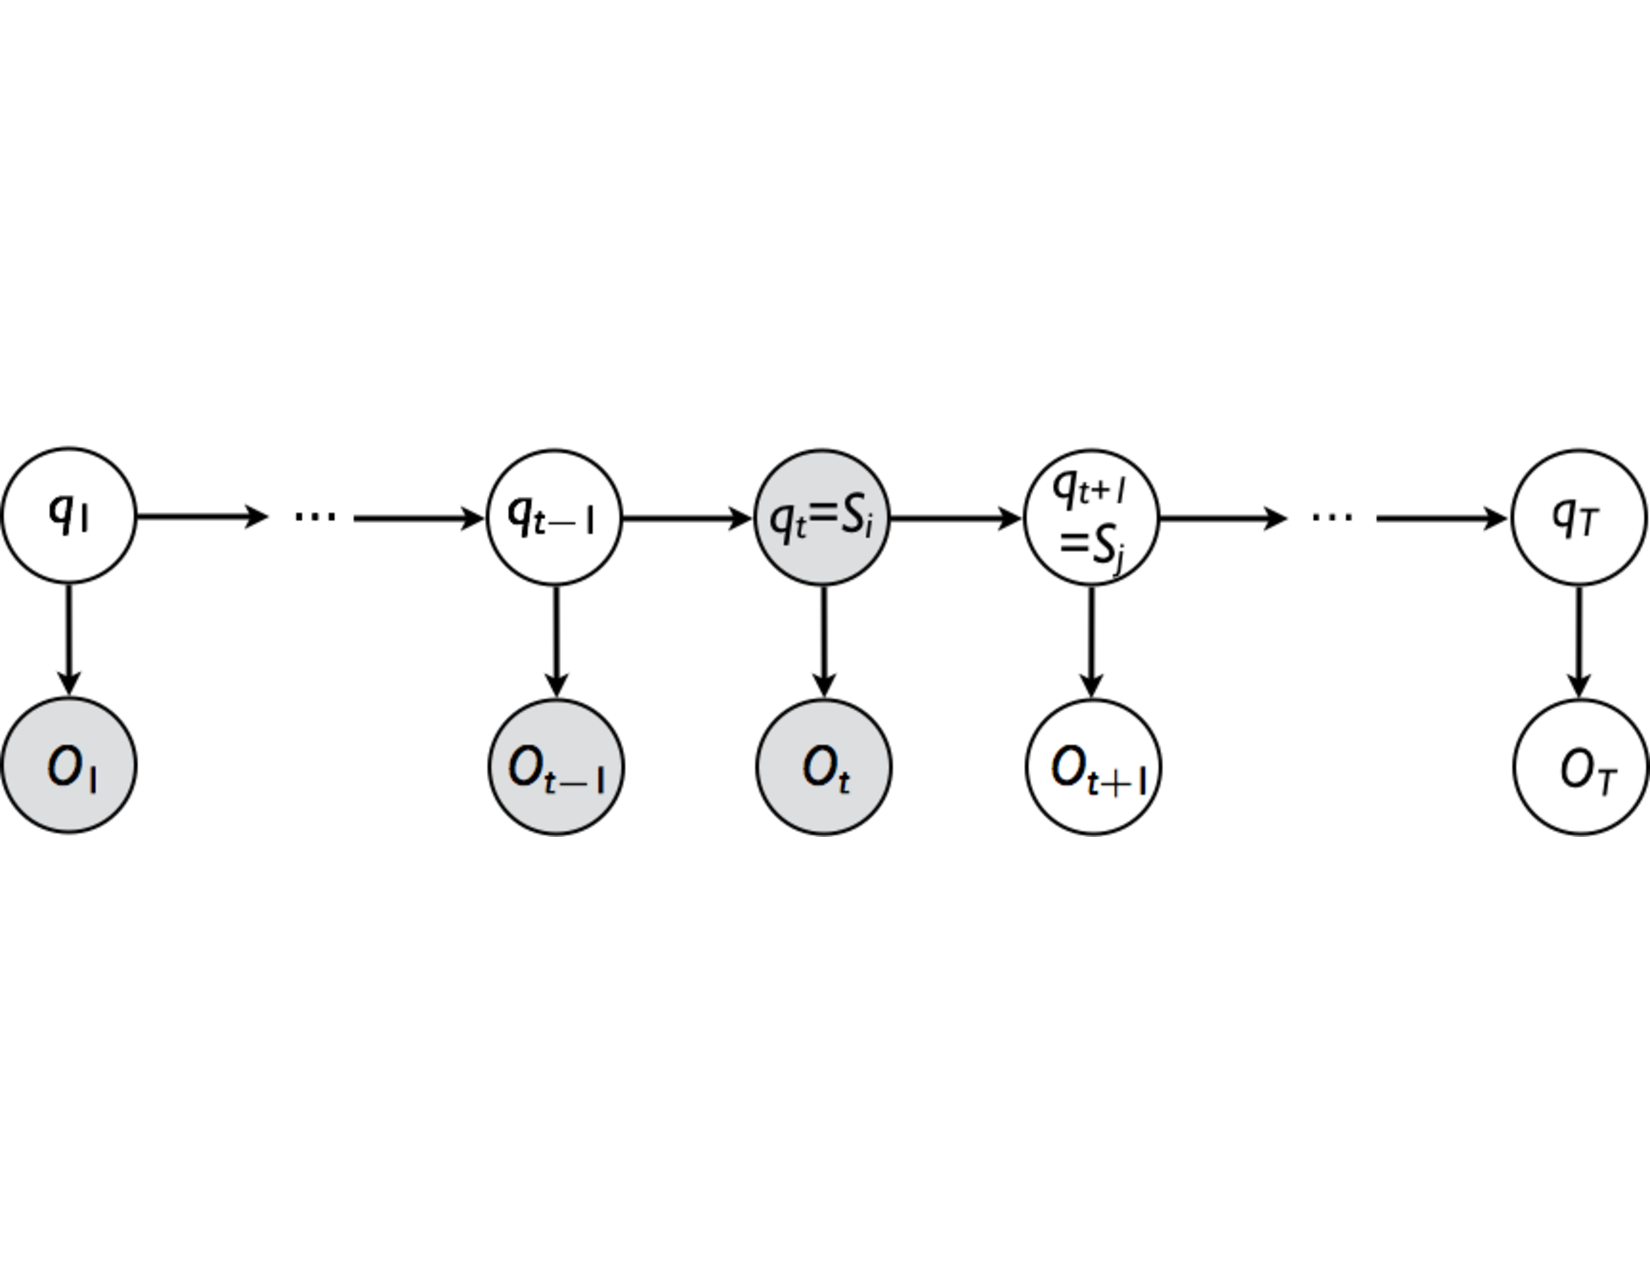
\includegraphics[width=12cm]{HMM.pdf}
\caption{Chaine de Markov cachée.}
\label{fig:hmm}
\end{figure}

%L'estimation des
%paramètres d'une chaine de Markov cachée à partir de séquences
%observées, est basée sur le calcul itératif de certaines probabilités,
%dont : 
%\begin{equation}\label{equ:beta}
%\beta_t(i) = P(O_{t+1}O_{t+2}\ldots O_T |q_t=S_i)
%\end{equation}
%Ici, $O_t$ est l'observation au temps $t$, $q_t$ est l'état caché au
%temps $t$ et $\{S_i\}_{i=1 \ldots K}$ est l'ensemble des états cachés. 


\section{Questions sur le papier ``Quantitative image analysis of
  cellular heterogeneity in breast tumors complements genomic profiling.''}

\question[2] DNA copy number profiling. Il existe des techniques
permettant de déterminer à partir d'un échantillon de cellules  le
nombre de copies d'un fragment d'ADN dans le génome de la cellule
étudiée. Cela permet entre autres d'identifier des duplications de
gènes. 
\begin{parts}
\part Quel est le problème de cette technique, quand on étudie un
échantillon provenant d'une tumeur~? 
\part Quelle est la stratégie proposée dans l'article pour corriger ce
problème~? 
\end{parts}

\question[4] Figure 5.A.   
\begin{parts}
\part Que décrivent les courbes de Kaplan-Meier telles que celles
présentées dans la Figure 5.A~? 
\part Comment les auteurs définissent-ils ``LI''~? 
\part Comment ont-ils séparé les tumeurs en ``LI low'' et ``LI high''
? 
\part Comment cette séparation se compare-t-elle à celle effectuée par
les médecins~? 
\end{parts}

\question[3] Figure 5.B
\begin{parts}
\part Que représentent les couleurs sur la figure 5.B~? 
\part Quelle propriété un classifieur capable de séparer les
survivants des décédés doit-il avoir~?
\end{parts}

\question[2] Figure 5.C. Dans la colonne de droite, on a utilisé le
classifieur de la figure 5.B pour séparer les tumeurs en deux groupes.  
\begin{parts}
\part Comment cette séparation se compare-t-elle à celle effectuée
uniquement sur la base des images ou encore celle effectuée uniquement
sur la base de signature d'expression des gènes~? 
\part Pourquoi les images peuvent-elles apporter une information
complémentaire à celle apportée par la mesure de l'expression des
gènes~?
\end{parts}

\question[1] Quels sont les descripteurs issus de l'anayse d'images que
les auteurs utilisent pour prédire la survie des patients~? 

\end{questions}

%\begin{enumerate}
%\item 
%\end{enumerate}
\end{document}
